In this section, we evaluate the performance of \name instantiation on
Cassandra. Our goal is to assess the suitability of \name for programming
loosely connected distributed applications. To this end, we first quantify the
overheads of implementing \name over Cassandra. Subsequently, we assess the
performance of MRDTs implemented using \name. And finally, we study the
performance of distributed build cache (Section~\ref{sec:motivation}).

\subsection{Experimental setup}

For the experiments, we use a Cassandra cluster with 4 nodes within the same
data center. Each Cassandra node runs on a baremetal Intel\textregistered
Xeon\textregistered E3-1240 CPU, with 4 physical cores, and 2 hardware threads
per core. Each core runs at 3.70GHz and has 128KB of L1 data cache, 128KB of L1
instruction cache, 1MB L2 cache and 8MB of L3 cache. Each machine has 32GB of
main memory. The machines are unloaded except for the Cassandra node. The ping
latency between the machines is 0.5ms on average. The clients are run on a
machine with the same configuration in the same data center.

For the experiments, Cassandra cluster is configured with a replication factor
of 1, read and write consistency levels of |ONE|. Hence, the cluster maintains
a single copy of each data item, and only waits for one of the servers to
respond to return the result of read and write to the client. These choices
lead to eventual consistency where the reads may not return the latest write.
The cluster may be configured with larger replication factor for better fault
tolerance. However, stronger consistency levels are not useful since \name
enforces per-key causal consistency over the underlying eventual consistency
offered by Cassandra. In fact, choosing strong consistency for reads and writes
in Cassandra does not offer strong consistency in \name since the visibility of
updates in \name is explicitly controlled with the use of |refresh| and
|publish|.

\subsection{Baseline overheads}

\begin{wrapfigure}{r}{0.55\textwidth}
	\vspace{-1cm}
	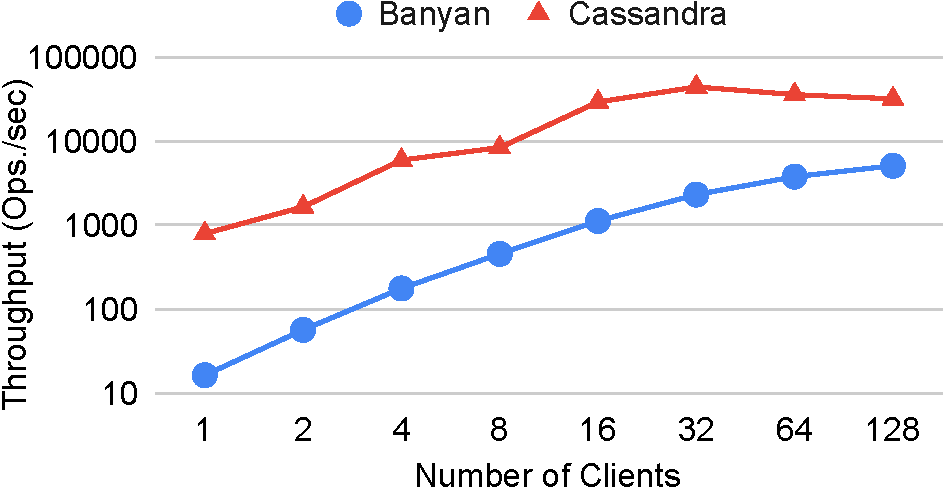
\includegraphics[scale=0.40]{results/baseline}
	\caption{Performance comparison between \name and Cassandra on LWW string
	value.}
	\label{res:baseline}
	\vspace{-0.5cm}
\end{wrapfigure}
Given that \name has to persist every version of the store, what is the impact
of \name when compared to using Cassandra in a scenario where Cassandra would
be sufficient? We measure the throughput of performing 32k operations, with
80\% reads and 20\% writes with different numbers of clients. The keys and
values are 8 and 128 byte strings, respectively. For \name, we use
last-writer-wins resolution policy, which is the policy used by Cassandra. The
results are presented in Figure~\ref{res:baseline}.

With 1 client, \name performs 16 operations per second, while Cassandra
performs 795 operations per second. Cassandra offers 50$\times$ more throughput
than \name with 1 client. This is due to the fact that every read (write)
performs 4 reads (3 reads and 4 writes) to the underlying store to create and
access the tag, commit and tree nodes. \name additionally includes marshalling
and hashing overheads for accessing the content-addressed block store.
Cassandra does not include any of these overheads. Luckily, \name overheads are
local to a client, and hence, can be easily parallelized. With 1 client, the
cluster is severely under utilized, and the client overheads dominate. With
increasing number of clients, the cluster is better utilized. At 128 clients,
Cassandra performs 31274 operations per second where as \name performs 5131
operations per second, which is a slowdown of 6.2$\times$. We believe that
these are reasonable overheads given the stronger consistency and isolation
guarantees, and better programming model offered by \name.

At the end of 32k operations, Cassandra uses 4.9MB of disk space, while \name
uses 1.8GB of disk space. As mentioned earlier (\S\ref{sec:gc}), we have yet to implement garbage collection for
\name -- once implemented, we expect this space usage will come down significantly.

\subsection{Mergeable Types}

\paragraph*{\textbf{Counter}} We begin with the counter data type discussed in
Section~\ref{sec:rec_merge}. How does \name counter perform on when
concurrently updated by multiple clients? For the experiment, the value type is
a counter that supports increment, decrement and read operations. The clients
perform 32k increment or decrement operations on a key randomly selected from a
small key space. Each client refreshes and publishes after every 100
operations. By choosing a small key space, we aim to study the scalability of
the system with large number of conflicts.

\begin{wrapfigure}{r}{0.55\textwidth}
	\vspace{-0.5cm}
	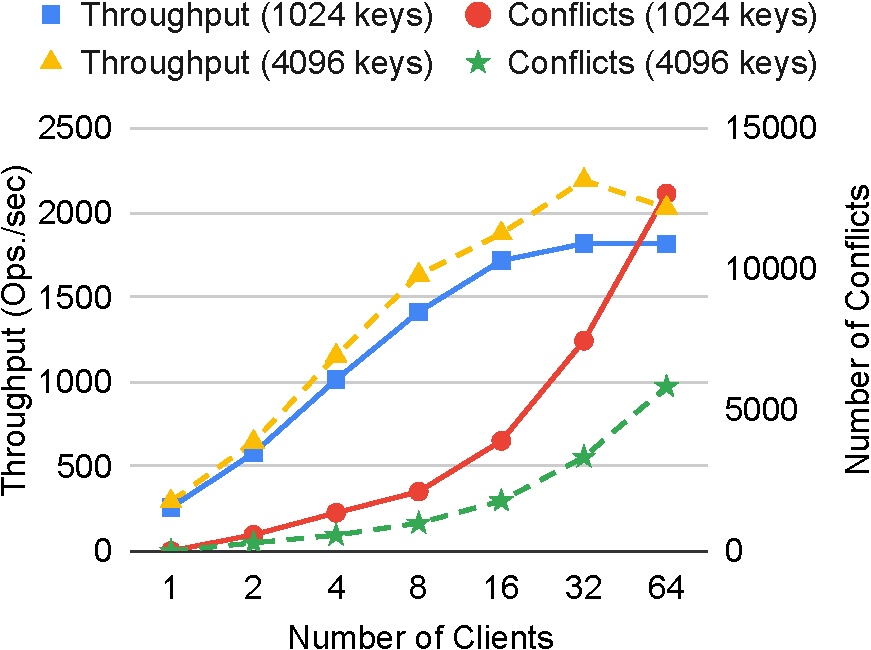
\includegraphics[scale=0.45]{results/counter}
	\caption{Performance of counter MRDT.}
	\label{res:counter}
	\vspace{-0.5cm}
\end{wrapfigure}
Figure~\ref{res:counter} shows the performance result for two key spaces of
size 1024 and 4096 keys. With 1 client, there are no conflicts. The conflicts
increases with increasing number of clients. We get a peak throughput of 1814
(2027) operations per second with a key space of 1024 (4096) keys. Observe that
the number of conflicts is considerably lower with 4096 keys when compared to
1024 keys. As a result, the throughput is higher with 4096 keys. The result
shows that the throughput of the system is proportional to the number of
conflicting operations.

\paragraph*{\textbf{Blob log}} Another useful class of MRDTs are
\emph{mergeable logs}, where each log message is a string. Such a distributed
log is useful for collecting logs in a distributed system, and examining the
logs in their global time order. To this end, each log entry is a pair of
timestamp and message, and the log itself is a list of such entries in reverse
chronological order. The merge function for the mergeable log extracts the
newer log entries from both the versions, sorts the newer entries in reverse
chronological order and returns the list obtained by appending the sorted newer
entries to the front of the log at the LCA.

While this implementation is simple, it does not scale well. In particular,
each commit stores the entire log as a single serialized blob. This does not
take advantage of the fact that every commit can share the tail of the log with
its predecessor. Moreover, every append to the log needs to deserialize the
entire log, append the new entry and serialize the log again. Hence, append is
an $O(n)$ operation, where $n$ is the size of the log. Merges are also worst
case $O(n)$. This is undesirable. We call this implementation a \emph{blob
log}.

\paragraph*{\textbf{Linked log}} We can implement a efficient logs by taking
advantage of the fact that every commit shares the tail of the log with its
predecessor. The value type in this log is:

\begin{lstlisting}
type value =
  | L of float (* timestamp *) * string (* message *)
	     * blob (* hash of prev value *)
	| M of blob list (* hashes of the values being merged *)
\end{lstlisting}

\begin{wrapfigure}{r}{0.4\textwidth}
	\vspace{-1cm}
	\centering
	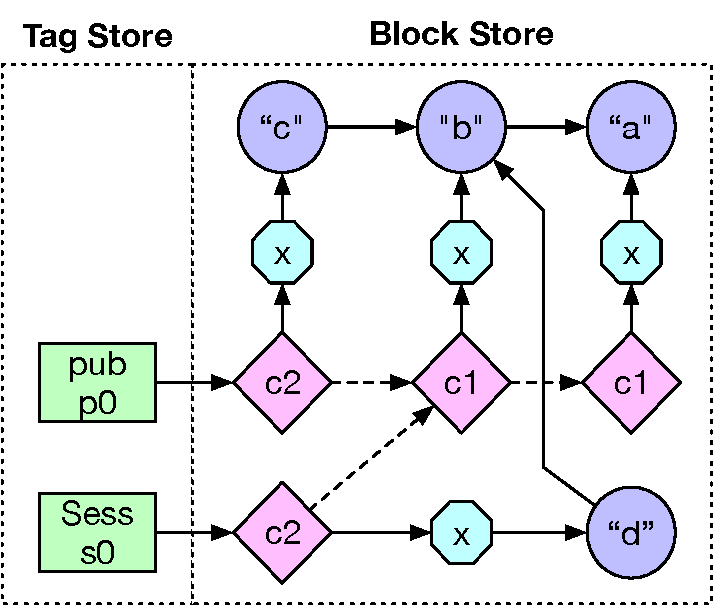
\includegraphics[scale=0.4]{figures/linked_log}
	\caption{A snapshot of linked log storage.}
	\label{fig:linked_log}
	\vspace{-0.5cm}
\end{wrapfigure}
The value is either a log entry |L(t,m,h)| with timestamp |t|, message |m| and
a hash of the previous value |h|. Appending to the log only needs to add a new
object that refers to the previous log value. Hence, append is $O(1)$.
Figure~\ref{fig:linked_log} shows a snapshot of the log assuming a single key
|x|. The log at |x| in the public branch |p0| (session |s0|) is |[a;b;c]|
(|[a;b;d]|). The merge operation simply adds a new value |M [h1;h2]|, which
refers to the hashes of the two log values being merged. This operation is also
$O(1)$. The read function for the log does the heavy-lifting of reading the log
in reverse chronological order.

\begin{wrapfigure}{l}{0.55\textwidth}
	\vspace{-0.5cm}
	\centering
	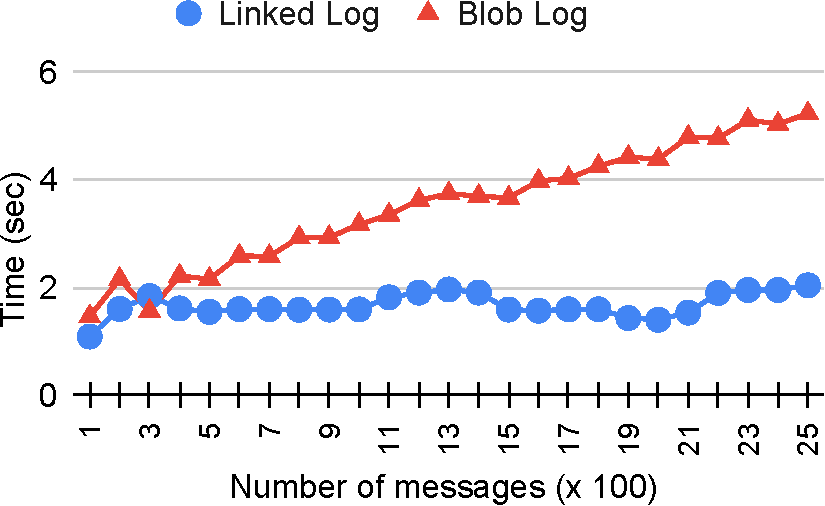
\includegraphics[scale=0.45]{results/log}
	\caption{Performance of mergeable logs.}
	\label{res:log}
	\vspace{-1.5cm}
\end{wrapfigure}
Observe that unlike the examples seen so far where the values do not refer to
other values, this \emph{linked log} implementation refers to other values as
heap data structures would do. Figure~\ref{res:log} shows the time taken to add
100 additional messages to the log with 4 clients. Observe that the time stays
constant with linked log but increases linearly with blob log. By being able to
share objects across different commits (versions), \name leads to efficient
implementations of useful data structures.

\subsection{Distributed build cache}

\begin{wrapfigure}{r}{0.45\textwidth}
	\vspace{-1cm}
	\centering
	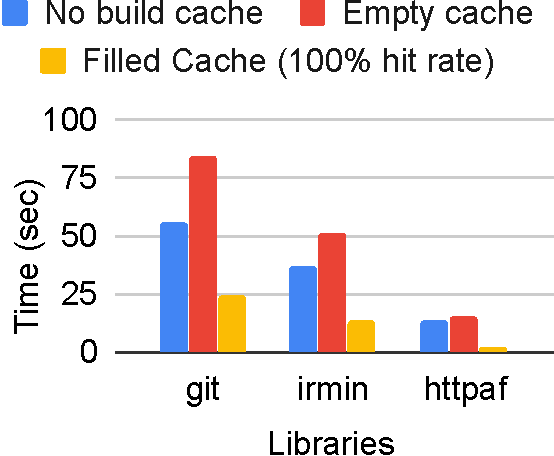
\includegraphics[scale=0.5]{results/build1}
	\caption{Performance of complete reuse of build artefacts.}
	\label{res:build1}
	\vspace{-0.5cm}
\end{wrapfigure}
In this section, we evaluate the performance of distributed build cache
described in Section~\ref{sec:motivation}. We have chosen three OCaml packages:
|git|, |irmin| and |httpaf| with common dependent packages. In the first
experiment, we measure the benefit of building a package that has already been
built in another workspace. Hence, the package artefacts will already be in the
build cache.

For each library, we measure the
baseline build time (1) without using the build cache, (2) using an empty build
cache, and (3) building the same package on a machine with the same package
having built earlier on a different machine. Figure~\ref{res:build1} shows the
results. We see that case using an empty build cache is slower than not using
the cache since the artefacts are stored in the cache. We also see that
building the same package on a different machine is faster due to the build
cache when compared to the baseline.

\begin{wrapfigure}{l}{0.45\textwidth}
	\vspace{-0.5cm}
	\centering
	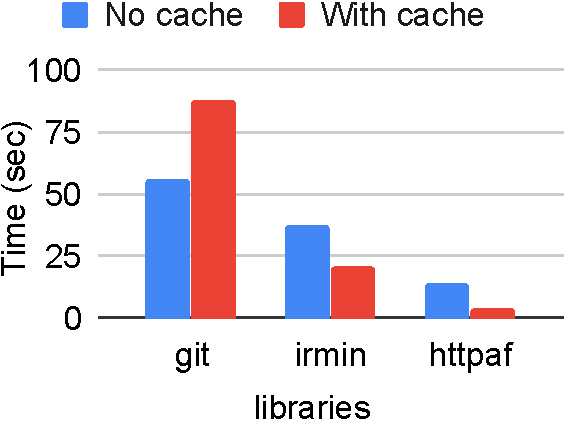
\includegraphics[scale=0.5]{results/build2}
	\caption{Performance of partial reuse of build artefacts.}
	\label{res:build2}
	\vspace{-0.5cm}
\end{wrapfigure}
A more realistic scenario is partial sharing of artefacts, where some of the
dependencies are in the cache and other need to be build locally, and added to
the cache. In this experiment, |git| package is first build on a machine with
an empty cache. Subsequently, |irmin| package is built on a second machine
(which will now benefit from the common artefacts in the cache). And finally,
building |httpaf| on a third machine, which benefits from both of the builds.
Figure~\ref{res:build2} shows the results. As expected, the |git| package build
is slower with cache than without since the cache is empty and the artefacts
need to be written to the cache additionally. Subsequent package builds benefit
from partial sharing of build artefacts. The results illustrate that \name not
only makes it easy to build complex applications like distributed build caches,
but the implementation also performs well under realistic workloads.
